\documentclass[letter,openrigh,12pt,spanish]{report}
\usepackage{amsfonts}
\usepackage{amsmath}
\usepackage{amssymb}
%Gummi|065|=)
\title{\textbf{Explicacion del Operador Jacobiano.}}
\author{Becerra I\~niguez Diego Armando\\
		Cinematica de Robots\\
		Ing. Mecatronica 7 A}
\date{15 de octubre de 2019}
\usepackage{graphicx}
\begin{document}

\maketitle

\section{Jacobiano}
En c\'alculo vectorial, se llama \textbf{jacobiano} o \textbf{determinante jacobiano} al determinar de la \textbf{matriz jacobiana}. Tanto la matriz jacobiana como el determinante jacobiano reciben su nombre en honor al matem\'atico Carl Gustav Jacobi.\\
En geometr\'ia algebraica, el \textbf{jacobiano} de una curva hace referencia a la variedad jacobiana, un grupo y variedad algebraica asociada a la curva, donde puede ser embebida.\\
La \textbf{matriz jacobiana} es una matriz formada por las derivadas parciales de primer orden de una funci\'on. Una de las aplicaciones m\'as interesantes de esta matriz es la posibilidad de aproximar linealmente a la funci\'on en un punto. En este sentido, el jacobiano representa la derivada de una funci\'on multivariable.\\
Propiamente deber\'iamos hablar m\'as que de matriz jacobiana, de \textbf{diferencial jacobiana} o \textbf{aplicaci\'on lineal jacobiana} ya que la forma de la amtriz dependera de la base o coordenadas elegidas. Es decir, dadas dos bases diferenciales la aplicaci\'on lineal jacobiana tendr\'a componentes diferenciales a\'un trat\'andose del mismo objeto matem\'atico. La propiedad b\'asica de la "matriz" jacobiana es la siguienes, dada una aplicaci\'on cualquiera \textbf{F:} $\mathbb{R}^N$ $\longrightarrow$ $\mathbb{R}^M$ continua, es decir:

\begin{displaymath}
\textbf{F}\in\textbf{C}^{(k)}(\mathbb{R}^N,\mathbb{R}^M)
\end{displaymath}
Se dira que es diferencial si exite una aplicaci\'on lineal \textbf{$\leftthreetimes$}$\in$\textbf{\textit{L}}($\mathbb{R}^N,\mathbb{R}^M$) tal que:

\begin{center}
\begin{displaymath}
\lim\limits_{||x-y|| \rightarrow 0} \frac{||\textbf{F(x)}-\textbf{F(y)}-\leftthreetimes(\textbf{x}-\textbf{y})||}{||\textbf{x}-\textbf{y}||}=0
\end{displaymath}
\end{center}

\section{Matriz Jacobiana de un campo vectorial}

Como \'ultimo caso particular de la noci\'on diferencial, suponemos ahora que el espacio normao de partida es $\mathbb{R}^N$ con N $\succ$ 1, y el de llegada es $\mathbb{R}^M$, tambien con M $\succ$ 1. Estudiando por tanto la diferenciabilidad de una funci\'on definida en uun abierto de $\mathbb{R}^N$ y con valores de N y M tenemos campos vectoriales muy variopintos, siendo l\'ogicamente N=M=2 Y N=M=3, los casos m\'as interesantes. Usando las bases usuales de $\mathbb{R}^N$ y $\mathbb{R}^M$, la diferencial de nuestra funci\'on en un punto, cuando existe, viene representada por una matriz M x N con coeficientes reales que ser\'a la \textit{matriz jacobiana}. Sus filas son los gradientes de M campos escalares en $\mathbb{R}^N$, las M componentes de nuestro campo vectorial. 

A la composici\'on de aplicaciones lineales corresponde entonces el producto de matrices, con lo que obtenemos una \textit{regla de la cadena para las derivadas parciales}. Como aplicaci\'on geom\'etria que merece destacarse, cuando N =2 y M=3 estudiamos el plano tangente a una \textit{superficie parametrica} en $\mathbb{R}^3$, generalizando lo que ya sabemos para superficies expl\'icitas.

\subsection{Matriz de una aplicaci\'on lineal}

Toda aplicaci\'on lineal T $\in$ L ($\mathbb{R}^N$, $\mathbb{R}^M$) admite una expresi\'on matricial que vamos a recordar. Denotamos por $\mathcal{M}_{MxN}$ al conjunto de todas la matrices M x N (M filas y N colummnas) con coeficientes reales, cuya estructura algebraica suponemos bien conocida. Para casa x $\in$$\mathbb{R}^N$, sus coordenadas $x_1$, $x_2$, ..., $x_N$ en la base usual de $\mathbb{R}^N$ forman una matriz colummna que tambi\'en denotamos por x, por lo que escribimos x $\in$$\mathcal{M}_{NX1}$. An\'alogamente, el vector y =T(x) $\in$$\mathbb{R}^M$ tiene sus coordenadas $y_1$, $y_2$, ..., $y_M$ en la base usual de $\mathbb{R}^M$, que forma la matriz columna y=T(x)como producto de matrices: y= \textbf{A}.x\\

De hecho, si escribimos A=($\alpha_{kj}$) para indicar los coeficientes de la matriz A, se tiene.

\begin{displaymath}
\alpha_{kj}=(\pi_k \circ T)(e_j) 	\forall \textbf{k}\in\textbf{\textit{I}}_M, \forall_j\in\textbf{\textit{I}}_N
\end{displaymath}

donde $e_j$ es el j-\'esimo vector de la base usual de $\mathbb{R}^N$ y $\pi_k$ la k-\'esima proyecci\'on coordenada en $\mathbb{R}^M$, tmabien con respecto a la base usual.

Diremos que A es la \textbf{la matriz de la aplicaci\'on lineal} \textit{T}, pero debemos entender su unicidad: es la \'unica matriz que representa a T en la forma y=A.x cuando, para x$\in$$\mathbb{R}^N$ y para y=T(x) $\in$ $\mathbb{R}^M$, usemos sus coordenadas bases usuales, escritas como matrices columna. Tenemos de hecho un isomorfismo entre los espacio vectoriales \textbf{L}($\mathbb{R}^N$,$\mathbb{R}^M$) y $\mathcal{M}_{MxN}$, que identifique cada \textbf{\textit{T}}$\in$ \textbf{L}($\mathbb{R}^N$,$\mathbb{R}^M$) con su matriz \textbf{A} $\in$ $\mathcal{M}_{MxN}$, reci\'en definida.

\subsection{Matriz Jacobiana}

En todo lo que sigue fijamos un abierto $\Omega$ de $\mathbb{R}^N$ y una funci\'on \textit{f}: $\Omega$ $\longrightarrow$ $\mathbb{R}^M$. Cuando M=1 tenemos un campo escalar en $\mathbb{R}^M$, los dos casos que ya hemos estudiando. Todo lo que hagamos ser\'a v\'alido en ambos casos, pero ahora nos interesa lo que ocurre cuando N $\succ$ 1 y M $\succ$ 1. Entonces se dice que \textit{f} es un \textbf{campo vectorial} y, si conviene precisar los valores de \textbf{M} y N, podemos decir que \textit{f} es un campo vectorial M-dimesional en N variables. Escribimos \textit{f}=($\textit{f}_1$,$\textit{f}_2$, ..., $\textit{f}_M$) para indicar las M componentes de \textit{f}, que son campos escalares como producto de matrices: y=\textbf{\textit{J}}\textit{f}(\textbf{$\alpha$}).x\\
De (1) deducimos que los coeficientes de las matriz jacobiana, \textbf{\textit{J}}\textit{f}($\alpha$)=($\alpha_kj$) $\in$ $\mathcal{M}_{MxN}$, viene dando por $\alpha_kj$=[$\pi_k\circ \textbf{D}\textit{f}(\alpha)$]($e_j$), para cualesquiera \textbf{k}$\in$$\textbf{\textit{I}}_M$ y \textit{j} $\in$$\textbf{texit{I}}_N$. Recordemos ahora que, para cada \textbf{k} $\in$$\textbf{textit{I}}_M$, la k-\'esima componente $\textit{f}_k$=$\pi
_k\circ \textit{f}$ es diferenciable en $\alpha$ con \textbf{D$\textit{f}_k$}($\alpha$)=$\pi_k\circ$\textbf{D}\textit{f}($\alpha$). Pero adem\'as, para todo \textit{j}$\in$$\textbf{\textit{I}}_N$, \textbf{D}$\textit{f}_k$($e_j$) es la derivada parcial de $\textit{f}_k$ con respecto a la \textit{j}-\'esima variable en el punto $\alpha$, luego

\begin{displaymath}
\alpha_kj=\textbf{D}\textit{f}_k(\alpha)(e_j)= \frac{\mathrm{d}\textit{f}_k}{\mathrm{d}\textit{x}_j}(\alpha)  \forall_k \in \textbf{\textit{I}}_M, \forall_j\in\textbf{\textit{I}}_N
\end{displaymath}

As\'i pues, la matriz jacobiana de \textit{f} en $\alpha$ viene dada por:\\

\begin{figure}[htp]
\centering
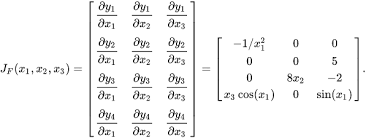
\includegraphics[scale=1]{1.png} 
\caption{Matriz}
\label{Figura}
\end{figure}

Se recuerda f\'acilmente, pues para cada \textbf{k} $\in$ $\textbf{\textit{I}}_M$, su k-\'esima fila es la gradiente de $\textit{f}_k$ en $\alpha$, es decir, las M filas de la matriz jacobiana son los gradientes de las M componentes de \textit{f}.\\
Cuando M=1, tenemos un campo escalar, cuya matriz jacobiana es su gradiente, escrito como una matriz fila, \textbf{\textit{J}}\textit{f}($\alpha$)=$\triangledown$ \textit{f}($\alpha$)$\in$ $\mathcal{M}_{1xM}$, de forma que, para todo x $\in$ $\mathbb{R}^N$, el producto escalar ($\triangledown$\textit{f}($\alpha$)|x) coincida con el producto de matrices \textbf{\textit{J}}\textit{f}($\alpha$).x=$\triangledown$\textit{f}($\alpha$).x. 

\bibliographystyle{apalike}
\bibliography{biblio}
\section{Referencias}
DE ROBOTS, A. D. C. (2017). INGENIERÍA MECATRÓNICA EN COMPETENCIAS PROFESIONALES.

Velázquez, J. G. R., Dıaz, E. O., y Dıaz, A. M. Modelo dinamico de un robot bıpedo planar de 9 grados de libertad en fase de vuelo y fases de contacto.

\end{document}